% Generated draft-margin slides: run Results/run_draft1944_analysis.R.
\begin{frame}[t]{1944 draft margins: internal and external response}
\tiny\centering
\begin{threeparttable}
\begin{tabular}{lccccc}
\toprule
 & Total internal & Retention & Same dept. & Diff. dept. & External hires \\
\midrule
Male drafted workers & 0.193$^{***}$ & 0.071$^{**}$ & 0.059$^{**}$ & 0.063$^{***}$ & 0.097$^{***}$ \\
 & (0.056) & (0.036) & (0.026) & (0.012) & (0.034) \\
\midrule
Observations & \multicolumn{5}{c}{623} \\
Offices clustered & \multicolumn{5}{c}{161} \\
Section and occupation FE & \multicolumn{5}{c}{Yes} \\
Log cumulative male baseline & \multicolumn{5}{c}{Yes} \\
\bottomrule
\end{tabular}
\begin{tablenotes}[flushleft]
\tiny\item \textit{Notes:} OLS, 1944 only. Unit: observed destination office $\times$ team $\times$ occupation cell, with section identifiers retained. Outcomes exclude male workers marked drafted in 1944. Exposure is the male draft count in the same office-team-occupation cell. Cells without observed non-draftee outcomes are outside the sample. These are conditional associations, not identified causal replacement effects. Internal total includes retention, same-department transfers, and different-department transfers. Standard errors clustered by office. $^{***}p<0.01$, $^{**}p<0.05$, $^{*}p<0.1$.
\end{tablenotes}
\end{threeparttable}
\vspace{2mm}
\par Internal / external $= 0.1932 / 0.0967 = \mathbf{2.00:1}$.
\end{frame}

\begin{frame}[t]{1944 draft margins: decomposition}
\centering
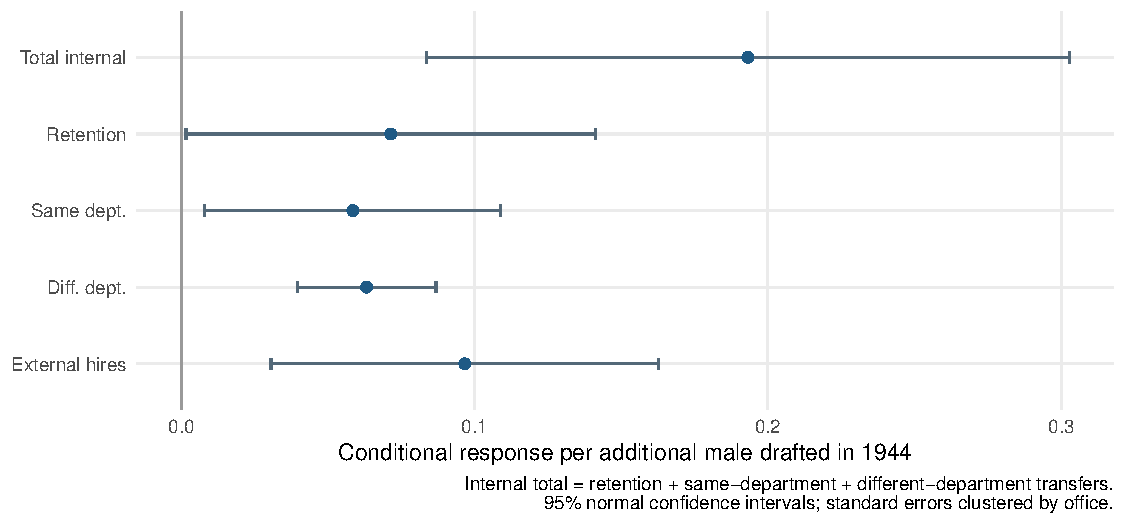
\includegraphics[width=0.92\textwidth]{Results/draft1944_pre_draft_trajectories/replacement_margins_1944.pdf}
\end{frame}

\begin{frame}[t]{Draft margins: pooled 1938--1945 benchmark}
\tiny\centering
\begin{threeparttable}
\begin{tabular}{lccccc}
\toprule
 & Total internal & Retention & Same dept. & Diff. dept. & External hires \\
\midrule
Male drafted workers & 0.408$^{***}$ & 0.227$^{***}$ & 0.100$^{**}$ & 0.081$^{***}$ & 0.206$^{**}$ \\
 & (0.076) & (0.073) & (0.040) & (0.015) & (0.100) \\
\midrule
Observations & \multicolumn{5}{c}{7,409} \\
Offices clustered & \multicolumn{5}{c}{1,192} \\
Section and occupation FE & \multicolumn{5}{c}{Yes} \\
Log cumulative male baseline & \multicolumn{5}{c}{Yes} \\
Year FE & \multicolumn{5}{c}{Yes} \\
\bottomrule
\end{tabular}
\begin{tablenotes}[flushleft]
\tiny\item \textit{Notes:} OLS benchmark over the 1938--1945 window (observed directories: 1938--1944), with year fixed effects. Exposure is the contemporaneous male draft count; this is not a 1944-only estimate. Internal total includes retention, same-department transfers, and different-department transfers. Standard errors clustered by office. $^{***}p<0.01$, $^{**}p<0.05$, $^{*}p<0.1$.
\end{tablenotes}
\end{threeparttable}
\vspace{2mm}
\par Internal / external $= 0.4079 / 0.2057 = \mathbf{1.98:1}$.
\end{frame}

\begin{frame}[t]{Post-merger entrant drafting: pooled benchmark}
\tiny\centering
\begin{threeparttable}
\begin{tabular}{lccccc}
\toprule
 & Total internal & Retention & Same dept. & Diff. dept. & External hires \\
\midrule
Male drafted workers & 0.465$^{*}$ & 0.221 & 0.096 & 0.148$^{***}$ & 0.335 \\
 & (0.246) & (0.188) & (0.070) & (0.042) & (0.243) \\
\midrule
Observations & \multicolumn{5}{c}{7,409} \\
Offices clustered & \multicolumn{5}{c}{1,192} \\
Section and occupation FE & \multicolumn{5}{c}{Yes} \\
Log cumulative male baseline & \multicolumn{5}{c}{Yes} \\
Year FE & \multicolumn{5}{c}{Yes} \\
\bottomrule
\end{tabular}
\begin{tablenotes}[flushleft]
\tiny\item \textit{Notes:} OLS over the 1938--1945 window (observed directories: 1938--1944), with year fixed effects. Exposure counts male post-merger entrants drafted in 1944; outcomes follow the pooled benchmark definition. Internal total includes retention, same-department transfers, and different-department transfers. Standard errors clustered by office. $^{***}p<0.01$, $^{**}p<0.05$, $^{*}p<0.1$.
\end{tablenotes}
\end{threeparttable}
\vspace{2mm}
\par Internal / external $= 0.4651 / 0.3354 = \mathbf{1.39:1}$.
\end{frame}

\begin{frame}[plain]\centering\vfill{\Large\bfseries Appendix}\vfill\end{frame}

\begin{frame}[t]{Draft intensity: total internal response DID}
    \scriptsize
    \centering
    \begin{threeparttable}
    \begin{tabular}{lccc}
        \toprule
        & Section + occ. + year FE & No section FE & No occ. FE \\
        \midrule
        No. future drafted $\times$ War & 2.120$^{***}$ & 2.352$^{***}$ & 2.085$^{***}$ \\
        & (0.682) & (0.822) & (0.657) \\
        No. future drafted $\times$ Mass drafting & -0.180 & -0.127 & -0.054 \\
        & (0.174) & (0.170) & (0.076) \\
        \midrule
        Observations & 936 & 988 & 938 \\
        Sections clustered & \multicolumn{3}{c}{173} \\
        Baseline male employment (log) & Yes & Yes & Yes \\
        \bottomrule
    \end{tabular}
    \begin{tablenotes}[flushleft]
        \tiny
        \item \textit{Notes:} Outcome: total internal response, including retention. Treatment: 1944 male draft count. Peace time, 1930--1936, is the omitted period; War is 1937--1943; Mass drafting is 1944. Standard errors clustered by section in parentheses. $^{***}p<0.01$, $^{**}p<0.05$, $^{*}p<0.1$.
    \end{tablenotes}
    \end{threeparttable}
\end{frame}

\begin{frame}[t]{Draft intensity: external hires DID}
    \scriptsize
    \centering
    \begin{threeparttable}
    \begin{tabular}{lccc}
        \toprule
        & Section + occ. + year FE & No section FE & No occ. FE \\
        \midrule
        No. future drafted $\times$ War & 0.925 & 0.911$^{*}$ & 1.015$^{*}$ \\
        & (0.561) & (0.527) & (0.578) \\
        No. future drafted $\times$ Mass drafting & 0.259$^{**}$ & 0.230$^{***}$ & 0.306$^{***}$ \\
        & (0.112) & (0.087) & (0.105) \\
        \midrule
        Observations & 936 & 988 & 938 \\
        Sections clustered & \multicolumn{3}{c}{173} \\
        Baseline male employment (log) & Yes & Yes & Yes \\
        \bottomrule
    \end{tabular}
    \begin{tablenotes}[flushleft]
        \tiny
        \item \textit{Notes:} Outcome: external hires. Treatment: 1944 male draft count. Peace time, 1930--1936, is the omitted period; War is 1937--1943; Mass drafting is 1944. Standard errors clustered by section in parentheses. $^{***}p<0.01$, $^{**}p<0.05$, $^{*}p<0.1$.
    \end{tablenotes}
    \end{threeparttable}
\end{frame}

\begin{frame}[t]{Total internal response: period DID}
    \scriptsize
    \centering
    \begin{threeparttable}
    \begin{tabular}{lccc}
        \toprule
        & Section + occ. + year FE & No section FE & No occ. FE \\
        \midrule
        Future drafted cell $\times$ War & 9.965$^{***}$ & 7.709$^{***}$ & 13.349$^{***}$ \\
        & (2.988) & (2.938) & (3.036) \\
        Future drafted cell $\times$ Mass drafting & -0.025 & 1.007$^{***}$ & 1.511$^{***}$ \\
        & (0.421) & (0.387) & (0.427) \\
        \midrule
        Observations & 10,108 & 10,286 & 10,111 \\
        Baseline male employment (log) & Yes & Yes & Yes \\
        \bottomrule
    \end{tabular}
    \begin{tablenotes}[flushleft]
        \tiny
        \item \textit{Notes:} Outcome: total internal response, including retention. Treatment: any male 1944 draftee in the cell. Peace time, 1930--1936, is the omitted period; War is 1937--1943; Mass drafting is 1944. Standard errors clustered by section in parentheses. $^{***}p<0.01$, $^{**}p<0.05$, $^{*}p<0.1$.
    \end{tablenotes}
    \end{threeparttable}
\end{frame}

\begin{frame}[t]{External hires: period DID}
    \scriptsize
    \centering
    \begin{threeparttable}
    \begin{tabular}{lccc}
        \toprule
        & Section + occ. + year FE & No section FE & No occ. FE \\
        \midrule
        Future drafted cell $\times$ War & 2.880 & 2.354 & 4.510$^{**}$ \\
        & (1.755) & (1.655) & (1.778) \\
        Future drafted cell $\times$ Mass drafting & -0.265 & 0.615$^{*}$ & 0.904$^{***}$ \\
        & (0.374) & (0.347) & (0.347) \\
        \midrule
        Observations & 10,108 & 10,286 & 10,111 \\
        Baseline male employment (log) & Yes & Yes & Yes \\
        \bottomrule
    \end{tabular}
    \begin{tablenotes}[flushleft]
        \tiny
        \item \textit{Notes:} Outcome: external hires. Treatment: any male 1944 draftee in the cell. Peace time, 1930--1936, is the omitted period; War is 1937--1943; Mass drafting is 1944. Standard errors clustered by section in parentheses. $^{***}p<0.01$, $^{**}p<0.05$, $^{*}p<0.1$.
    \end{tablenotes}
    \end{threeparttable}
\end{frame}

\begin{frame}[t]{Draft intensity: total internal yearly associations}
\centering
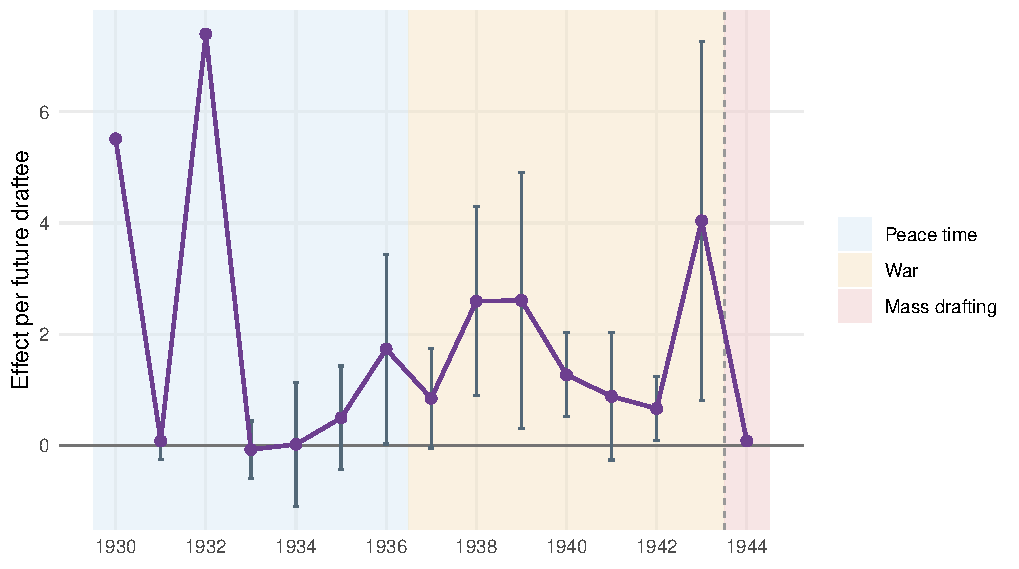
\includegraphics[width=0.84\textwidth]{Results/draft1944_pre_draft_trajectories/draft_intensity_treatment_internal.pdf}
\parbox{0.9\textwidth}{\centering\tiny Separate year-by-year conditional associations with 1944 draft exposure; section and occupation FE and log cumulative male control. Bars show 95\% normal confidence intervals.}
\end{frame}

\begin{frame}[t]{Draft intensity: external hires yearly associations}
\centering
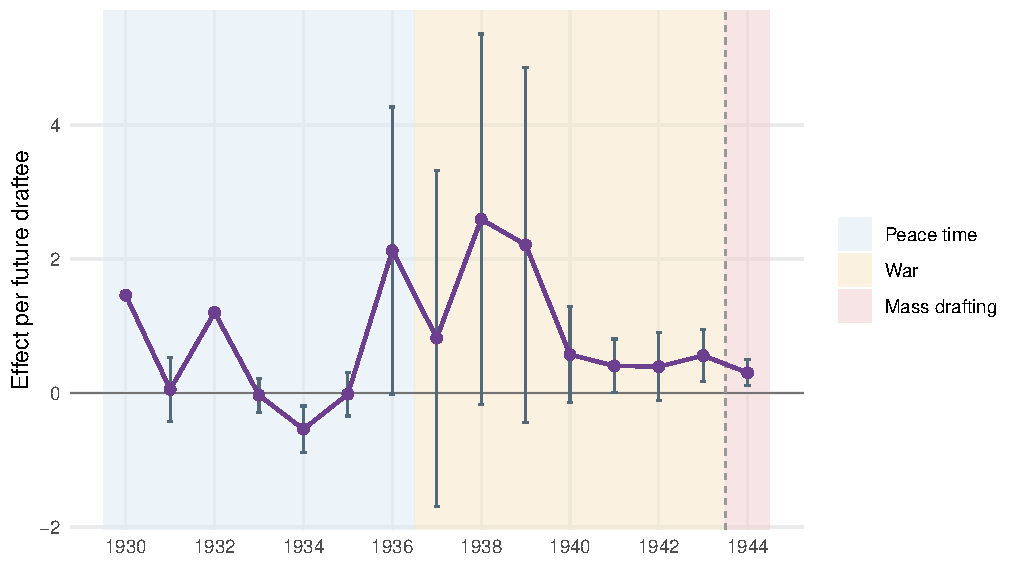
\includegraphics[width=0.84\textwidth]{Results/draft1944_pre_draft_trajectories/draft_intensity_treatment_new_hires.pdf}
\parbox{0.9\textwidth}{\centering\tiny Separate year-by-year conditional associations with 1944 draft exposure; section and occupation FE and log cumulative male control. Bars show 95\% normal confidence intervals.}
\end{frame}

\begin{frame}[t]{Total internal response: yearly associations}
\centering
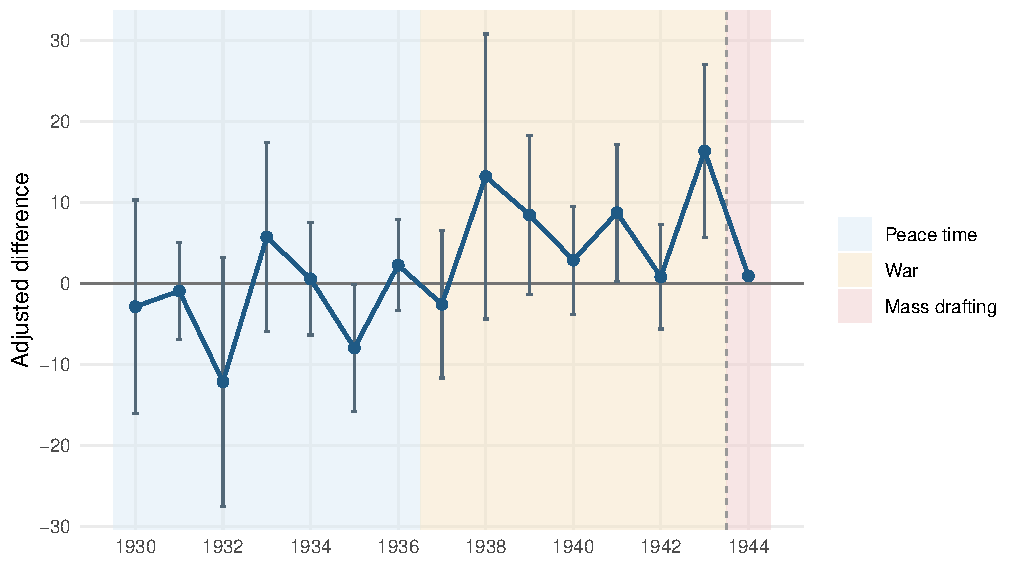
\includegraphics[width=0.84\textwidth]{Results/draft1944_pre_draft_trajectories/within_section_pretrend_internal.pdf}
\parbox{0.9\textwidth}{\centering\tiny Separate year-by-year conditional associations with 1944 draft exposure; section and occupation FE and log cumulative male control. Bars show 95\% normal confidence intervals.}
\end{frame}

\begin{frame}[t]{External hires: yearly associations}
\centering
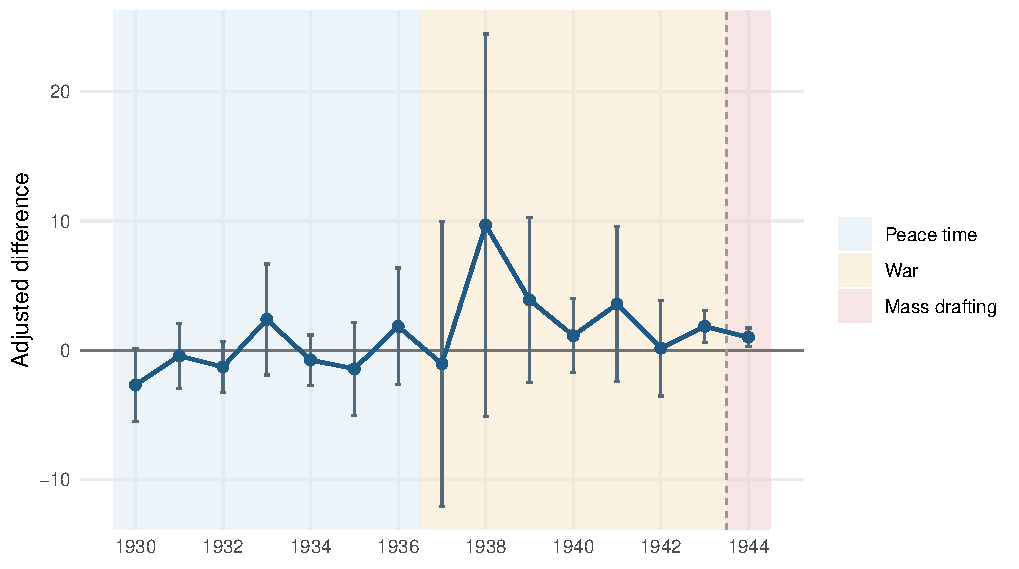
\includegraphics[width=0.84\textwidth]{Results/draft1944_pre_draft_trajectories/within_section_pretrend_new_hires.pdf}
\parbox{0.9\textwidth}{\centering\tiny Separate year-by-year conditional associations with 1944 draft exposure; section and occupation FE and log cumulative male control. Bars show 95\% normal confidence intervals.}
\end{frame}


\begin{frame}[t]{Bilateral mobility: nested organizational distance}
    \small
    \vspace{0.4em}
    \textbf{Unit:} origin office $\times$ origin occupation $\times$ destination office $\times$ destination occupation $\times$ year.

    \vspace{0.8em}
    \begin{align*}
    E[F_{o p, d q, t}] =
    \exp\{&
        \beta_1 \log N_{o p,t-1}
        + \beta_2 \log N_{d q,t-1}
        + \beta_3 \log N_{o p,t-1}\log N_{d q,t-1} \\
        &+ \beta_4 \mathrm{OccSimilarity}_{od,t-1}
        + \beta_5 \mathbf{1}\{\mathrm{same\ kyoku,\ diff.\ ka}\}
        + \beta_6 \mathbf{1}\{\mathrm{diff.\ kyoku}\}
        + \alpha_t + \Gamma
    \}
    \end{align*}

    \vspace{0.4em}
    \begin{itemize}
        \item Retention is same office and same occupation; excluded from the flow panel.
        \item Baseline category: workers change occupation within the same ka $\times$ kyoku.
        \item \textbf{Same kyoku, different ka}: within-department cross-section mobility.
        \item \textbf{Different kyoku}: cross-department mobility. Sample excludes office-years with drafting at either endpoint.
    \end{itemize}
\end{frame}

\begin{frame}[t]{Bilateral mobility: strong nested distance gradient}
    \centering
    \tiny
    \setlength{\tabcolsep}{3.2pt}
    \begin{threeparttable}
    \begin{tabular}{lcccccc}
        \toprule
        & (1) & (2) & (3) & (4) & (5) & (6) \\
        & Year FE & Occ-pair FE & Origin kyoku FE & Dest. kyoku FE & Origin ka FE & Dest. ka FE \\
        \midrule
        $\log N_{o,p}$ & 0.778$^{***}$ & 0.861$^{***}$ & 0.773$^{***}$ & 0.781$^{***}$ & 0.855$^{***}$ & 0.763$^{***}$ \\
        & (0.075) & (0.099) & (0.077) & (0.076) & (0.074) & (0.092) \\
        $\log N_{d,q}$ & 0.239$^{***}$ & 0.130 & 0.218$^{***}$ & 0.222$^{***}$ & 0.163$^{**}$ & 0.151$^{**}$ \\
        & (0.060) & (0.099) & (0.062) & (0.064) & (0.072) & (0.066) \\
        $\log N_{o,p}\times \log N_{d,q}$ & 0.007 & -0.041 & 0.012 & 0.010 & 0.036 & 0.031 \\
        & (0.019) & (0.027) & (0.019) & (0.019) & (0.025) & (0.025) \\
        Occupation similarity & 1.788$^{***}$ & 1.090$^{***}$ & 1.536$^{***}$ & 1.404$^{***}$ & 1.574$^{***}$ & 1.296$^{***}$ \\
        & (0.359) & (0.381) & (0.366) & (0.384) & (0.371) & (0.422) \\
        Same kyoku, diff. ka & -2.334$^{***}$ & -3.519$^{***}$ & -2.324$^{***}$ & -2.375$^{***}$ & -2.361$^{***}$ & -2.408$^{***}$ \\
        & (0.326) & (0.339) & (0.346) & (0.358) & (0.340) & (0.344) \\
        Different kyoku & -4.659$^{***}$ & -5.889$^{***}$ & -4.860$^{***}$ & -4.943$^{***}$ & -4.897$^{***}$ & -5.025$^{***}$ \\
        & (0.271) & (0.272) & (0.298) & (0.287) & (0.290) & (0.290) \\
        \midrule
        Observations & 4,445,908 & 2,684,319 & 4,406,699 & 3,590,943 & 2,778,413 & 1,420,716 \\
        Pseudo $R^2$ & 0.333 & 0.416 & 0.352 & 0.357 & 0.389 & 0.410 \\
        \bottomrule
    \end{tabular}
    \begin{tablenotes}[flushleft]
        \tiny
        \item \textit{Notes:} PPML regressions. Unit is origin office--occupation $\times$ destination office--occupation $\times$ year, 1938--1945. Retention, defined as same office and same occupation, is excluded. Omitted category is same office (ka $\times$ kyoku), different occupation. A literal same-kakari baseline has no positive flow cells in the kakari-covered sample. Standard errors clustered two-way by origin and destination office. $^{***}p<0.01$, $^{**}p<0.05$, $^{*}p<0.1$.
    \end{tablenotes}
    \end{threeparttable}
\end{frame}

\begin{frame}[t]{Selection into draft-induced vacancies}
    \centering
    \tiny
    \resizebox{\linewidth}{!}{%
    \begin{tabular}{lcccccc}
        \toprule
         & \multicolumn{2}{c}{All transfers} & \multicolumn{2}{c}{Different ka, same kyoku} & \multicolumn{2}{c}{Different kyoku} \\
        \cmidrule(lr){2-3} \cmidrule(lr){4-5} \cmidrule(lr){6-7}
         & Any: Draft Vac. & Any: Non-Draft & Diff Ka: Draft & Diff Ka: Non-Draft & Diff Kyoku: Draft & Diff Kyoku: Non-Draft \\
        \midrule
        Decoration rank (0--8; high=better) & -0.0529 & 0.2466 & -15.4652$^{***}$ & 0.2863 & 0.1670 & 0.2020 \\
                               & (0.4393) & (0.1728) & (0.0000) & (0.1787) & (0.4425) & (0.2030) \\[3pt]
        Court rank (0--8; high=better) & -0.0186 & -0.1181$^{**}$ & -0.3238 & -0.0864 & 0.0372 & -0.1504$^{**}$ \\
                          & (0.1355) & (0.0601) & (0.3940) & (0.0667) & (0.1420) & (0.0734) \\[3pt]
        Female & -1.0508 & 0.3935$^{*}$ & -18.5681$^{***}$ & 0.4252$^{*}$ & -0.6950 & 0.3173 \\
               & (0.8136) & (0.2358) & (0.0000) & (0.2467) & (0.8277) & (0.2850) \\[3pt]
        Tenure (yrs) & 0.1014$^{***}$ & 0.0295$^{**}$ & -0.0950$^{**}$ & -0.0209 & 0.2123$^{***}$ & 0.0965$^{***}$ \\
                     & (0.0223) & (0.0125) & (0.0414) & (0.0139) & (0.0258) & (0.0145) \\[3pt]
        Log salary (prior year) & -0.1404 & -0.2396$^{***}$ & 0.1765 & -0.1763$^{*}$ & -0.3365$^{*}$ & -0.3171$^{***}$ \\
                        & (0.1625) & (0.0921) & (0.2320) & (0.1012) & (0.1891) & (0.1050) \\[3pt]
        \midrule
        Year FE & \multicolumn{6}{c}{Yes} \\
        Observations & \multicolumn{6}{c}{5,523} \\
        Log-likelihood & \multicolumn{2}{c}{-3140.5} & \multicolumn{4}{c}{-5295.7} \\
        AIC & \multicolumn{2}{c}{6329.1} & \multicolumn{4}{c}{10687.5} \\
        \bottomrule
    \end{tabular}}
    \vspace{0.5em}

    {\tiny Sample restricted to origin office-unit $\times$ year cells with at least one transfer to a different ka or kyoku, further restricted to workers with observed prior-year salary. Base category: stayed in same ka and kyoku (required for MNL interpretation). Rank variables are coded 0--8, with higher values indicating higher status.}
\end{frame}


\begin{frame}{Trajectory regression: transferees vs peers}
    \scriptsize
    \begin{table}
    \centering
    \begin{tabular}{lcccc}
        \tabularnewline \midrule \midrule
                                                        & Tenure after   & Postwar surv.  & Postwar years  & Rank gain      \\
        \midrule
        \uncover<2->{\textbf{Transferred} vs.\ workers who \textbf{stayed at donor}}
                                                        & \uncover<2->{3.7525$^{***}$} & \uncover<2->{0.1953$^{***}$} & \uncover<2->{0.6345$^{***}$} & \uncover<2->{0.1813$^{***}$} \\
                                                        & \uncover<2->{(0.0911)}       & \uncover<2->{(0.0052)}       & \uncover<2->{(0.0206)}       & \uncover<2->{(0.0071)}       \\[4pt]
        \uncover<3->{\textbf{Draft-induced} vs.\ \textbf{natural-exit} destination}
                                                        & \uncover<3->{1.5513$^{***}$} & \uncover<3->{0.0801$^{***}$} & \uncover<3->{0.4697$^{***}$} & \uncover<3->{0.0304$^{**}$}  \\
                                                        & \uncover<3->{(0.2350)}       & \uncover<3->{(0.0153)}       & \uncover<3->{(0.0649)}       & \uncover<3->{(0.0137)}       \\[4pt]
        \uncover<4->{\textbf{Transferred} vs.\ workers \textbf{already at destination}}
                                                        & \uncover<4->{2.2992$^{***}$} & \uncover<4->{0.1426$^{***}$} & \uncover<4->{0.4895$^{***}$} & \uncover<4->{0.1348$^{***}$} \\
                                                        & \uncover<4->{(0.0868)}       & \uncover<4->{(0.0059)}       & \uncover<4->{(0.0208)}       & \uncover<4->{(0.0060)}       \\
        \midrule
        \emph{Fixed-effects}\\
        Team                       & Yes            & Yes            & Yes            & Yes            \\
        Occupation                 & Yes            & Yes            & Yes            & Yes            \\
        Year                       & Yes            & Yes            & Yes            & Yes            \\
        \midrule
        Observations               & \multicolumn{4}{l}{Row 1: 91,586 \quad Row 2: 40,060 \quad Row 3: 97,145} \\
        \midrule \midrule
        \multicolumn{5}{l}{\emph{Clustered SE in parentheses; ***: 0.01, **: 0.05, *: 0.1}}\\
    \end{tabular}
    \end{table}
\end{frame}

\begin{frame}{Promotion and bonus salary responses}
    \scriptsize
    \begin{table}
    \centering
    \begin{tabular}{lcccc}
        \tabularnewline \midrule \midrule
        & \multicolumn{2}{c}{\textit{No.\ promoted workers}}
        & \multicolumn{2}{c}{\textit{No.\ bonus recipients}} \\
        \cmidrule(lr){2-3}\cmidrule(lr){4-5}
        Model:                           & (1)            & (2)            & (3)            & (4)            \\
        \midrule
        \emph{Variables}\\
        No.\ drafted workers             & 0.0267$^{*}$   & 0.0231$^{*}$   & 0.1367$^{**}$  & 0.1548$^{***}$ \\
                                         & (0.0107)       & (0.0114)       & (0.0529)       & (0.0587)       \\
        No.\ drafted $\times$ Part-time  &                & 0.0154         &                & $-0.1854^{**}$ \\
                                         &                & (0.0112)       &                & (0.0610)       \\
        \midrule
        \emph{Fixed-effects}\\
        Year / Section / Occupation      & Yes            & Yes            &                &                \\
        Section / Occupation             &                &                & Yes            & Yes            \\
        Log section size                 & Yes            & Yes            & Yes            & Yes            \\
        \midrule
        Observations                     & 2,770          & 2,770          & 576            & 576            \\
        \midrule \midrule
        \multicolumn{5}{l}{\emph{Clustered SE in parentheses; ***: 0.01, **: 0.05, *: 0.1}}\\
    \end{tabular}
    \end{table}
\end{frame}
